%=====================================================================================================
\section{Method}
\figif{fig_architecture.pdf}{%
\begin{figure*}[t]
\centering
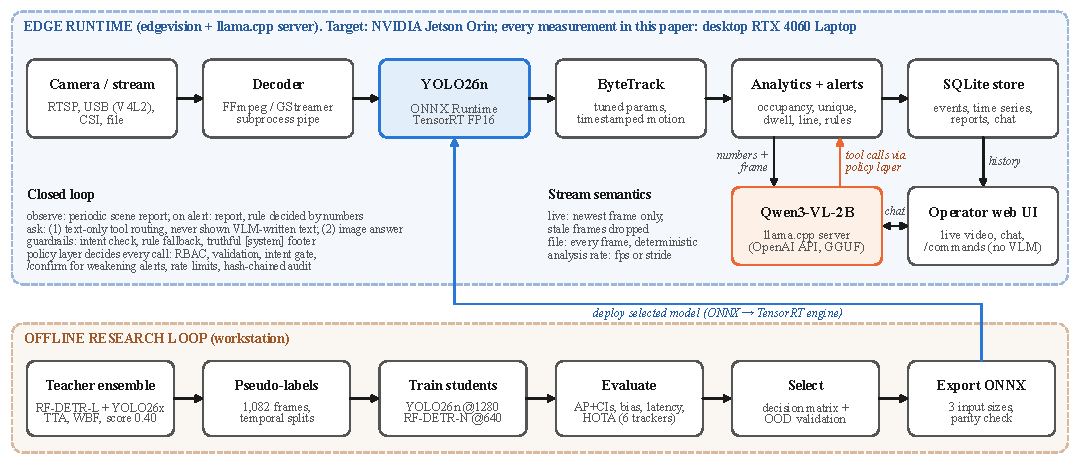
\includegraphics[width=\textwidth]{figures/fig_architecture.pdf}
\caption{System overview. Top: the edge runtime (target: Jetson Orin; measured here on a desktop GPU); detections
flow left to right, the VLM receives the live analytics and frame and acts back on the analytics only through tool
calls that a deterministic policy layer decides. Bottom: the offline loop that labels, trains, evaluates, selects and
exports the detector.}
\label{fig:arch}
\end{figure*}}

\subsection{Scenes and pseudo-labels}
\label{sec:data}
\textbf{aa1 (adaptation scene).} From the 300\,s, 59.94\,fps, $1280{\times}720$ handheld plaza video we sample one
frame every 0.25\,s between 30\,s and 300\,s (1,082 frames). Each frame is labelled by RF-DETR Large and YOLO26x
(test-time augmentation, $1280$\,px), both at score $\geq 0.15$; their boxes are fused by WBF (IoU 0.55, equal
weights, averaged scores) and fused boxes with score $\geq 0.40$ are kept. The splits are contiguous in time:
train 30--210\,s (\ImgsTrain{} frames, \BoxesTrain{} boxes), valid 210--255\,s (\ImgsValid{}/\BoxesValid{}), test
255--300\,s (\ImgsTest{}/\BoxesTest{}); the first 30\,s are reserved for tracking (Fig.~\ref{fig:data}).

\textbf{Three campus scenes.} Two $1920{\times}1080$ phone videos of other campus locations (\emph{scene~1}: people
walking past a building close to the camera; \emph{scene~2}: a camera at ground level against the light; about
200\,s each) are labelled with the same recipe on every frame and split in time (train first 60\,\%, valid 15\,\%,
test last 25\,\%); they serve as extra adaptation scenes, validation scenes and test scenes. The held-out
\emph{test1} video (a tree-lined road from a fixed position, 298\,s) is used \emph{only for testing}: nothing is
trained, tuned, thresholded or selected on it.

\textbf{COCO people.} The two halves of COCO val2017 (human labels; not seen by the COCO-pretrained students) give a
replay pool (720 images, 15\,\% without people) and a disjoint 600-image person validation set used to measure
forgetting and to choose blend weights.

\figif{fig_dataset.pdf}{%
\begin{figure}[t]
\centering
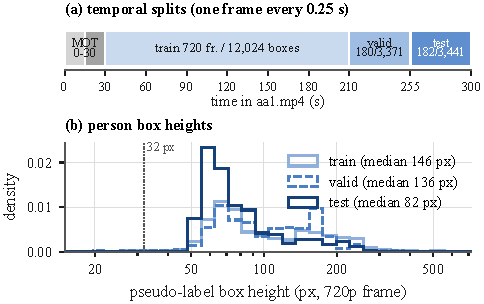
\includegraphics[width=\columnwidth]{figures/fig_dataset.pdf}
\caption{(a) Temporal use of \texttt{aa1}: tracking hold-out (0--15\,s tuning, 15--30\,s evaluation) and the
detection splits. (b) Pseudo-label box heights per split.}
\label{fig:data}
\end{figure}}

\subsection{Students and adaptation variants}
\label{sec:variants}
\yolo{} (COCO-pretrained, 2.5\,M parameters) is fine-tuned for 150 epochs at 1280\,px (AdamW set explicitly, lr
$10^{-3}$, cosine schedule, batch 12, seed 0). \rfdetr{} is fine-tuned at 640\,px for 80 epochs (EMA, cosine,
effective batch 16, lr $10^{-4}$, encoder $1.5{\times}10^{-4}$). These are each model's \emph{deployment}
configurations; the architecture comparison at matched input size is in Sec.~\ref{sec:res}.

For the adaptation study all \yolo{} variants keep the 80-class COCO head (person = class 0) so that their weights
remain shape-compatible with the pretrained model, and differ from the reference \emph{FT-aa1} (aa1 labels, same
recipe) in one respect each: \emph{replay} adds the 720 COCO replay images (1:1, as in
Scenes100~\cite{zhang2023scenes100}); \emph{frozen} freezes the 11 backbone modules (lr $3{\times}10^{-4}$, 40
epochs); \emph{ignore} greys out every fused teacher box with $0.15\le s<0.40$ that overlaps no kept label, so
uncertain people are neither positives nor background; \emph{multi-scene} trains on aa1 + scene~1 + scene~2;
\emph{scene~1}/\emph{scene~2} train on one campus scene; \emph{FT@640} trains at 640\,px. \textbf{WiSE.} For
$\alpha\in\{0,0.1,\dots,1\}$ the blend $\theta(\alpha)=(1-\alpha)\,\theta_{\text{pre}}+\alpha\,\theta_{\text{FT}}$ is
evaluated with linearly blended BatchNorm statistics and with statistics re-estimated on 192 training-time images
(aa1 train + COCO replay)~\cite{wortsman2022wise,medeiros2026wiseod}; $\alpha$ is chosen on aa1-valid and COCO-val
only.

\subsection{Evaluation protocol}
All models are scored with one script on every split and scene. \emph{COCO metrics}~\cite{lin2014coco}: \AP{},
\APf{}, \APs{}, AP by size, AR@300. \emph{Operating point}: the best-F1 confidence threshold on the model's own
training-scene validation split, frozen everywhere else; P/R/F1 at IoU 0.5, FPPI, LAMR~\cite{dollar2012pedestrian},
per-frame counting MAE and recall by person height. \emph{Label bias}: predictions are re-scored against each
teacher alone. \emph{Overfitting}: the train--test gap of a fine-tuned model minus that of its pretrained
counterpart. \emph{Cross-check}: headline numbers are recomputed by code sharing nothing with the evaluator.
% Statistical protocol (review items 5 and 13): units, resampling, p-values.
\subsection{Statistical protocol}
\label{sec:stats}
\textbf{Units.} We distinguish four units (Table~\ref{tab:units}). Frames 0.25\,s apart from one video are
\emph{observations}, not independent replicates: the same people appear in neighbouring frames in nearly the same
places. Uncertainty from frame sampling is therefore estimated by resampling contiguous \emph{blocks} of frames, and
claims about other cameras are supported only by additional \emph{scenes}; a frame-level interval says nothing about
scene-to-scene variation.

\begin{table}[t]
\centering
\caption{Experimental units and how each enters the statistics.}
\label{tab:units}
\footnotesize
\setlength{\tabcolsep}{2.5pt}
\begin{tabular}{p{0.15\columnwidth}p{0.36\columnwidth}p{0.41\columnwidth}}
\toprule
Unit & What it is & Used for \\
\midrule
Frame & one sampled image (0.25\,s apart) & observation; AP, F1, counts are pooled over frames \\
Block & $b$ consecutive frames (2.5/5/10\,s) & resampling unit of the CIs and paired tests \\
Track & one identity over time & HOTA/IDF1; 30\,s segments for paired tracker tests \\
Scene & one video / camera & generalisation claims; one replicate per scene \\
\bottomrule
\end{tabular}
\end{table}

\textbf{Resampling.} AP is not a per-frame mean, so every replicate re-pools the cached per-frame matches of the
resampled frames and recomputes the 101-point AP (the PASCAL~VOC practice~\cite{everingham2015voc}, with blocks
instead of images). The primary scheme, fixed before the analysis, is the paired circular block
bootstrap~\cite{politis1992cbb} with 5\,s blocks (20 frames) and $B{=}\TcB$ replicates shared by all models;
i.i.d.\ frames, 2.5\,s and 10\,s blocks, the moving-block bootstrap~\cite{kunsch1989} and the Politis--White
automatic block length~\cite{politis2004block,patton2009correction} (computed on the per-frame TP and FP series)
are sensitivity analyses. Intervals are percentile intervals.

\textbf{p-values.} A paired difference $\Delta$ between two models is tested by inverting the bootstrap interval
of $\Delta^*$: $p = \min\{1,\,2\min[(k_{\le 0}{+}1)/(B{+}1),\,(k_{\ge 0}{+}1)/(B{+}1)]\}$, where $k_{\le 0}$
($k_{\ge 0}$) counts replicates with $\Delta^*\le 0$ ($\ge 0$). The $+1$ terms are the finite-sample
correction~\cite{phipson2010pvalues}, so $p$ is never zero and its floor is $2/(B{+}1)$; a result at the floor is
written $p\le 2/(B{+}1)$. Wilcoxon tests are applied only to 30\,s segments and McNemar tests only to tracks, never
to correlated frames~\cite{dror2018hitchhiker}.


\subsection{Tracking}
Tracking is evaluated on the unseen first 30\,s of aa1 at the full frame rate (\GtFrames{} frames) and on whole
test videos. Pseudo-GT tracks link teacher detections with ByteTrack (activation 0.40, buffer \GtBuffer{} frames,
tracks $\geq$0.25\,s). ByteTrack parameters are grid-searched per detector on aa1 0--15\,s (\GridSize{}
configurations) and reported on 15--30\,s; six trackers (\texttt{trackers} library~\cite{trackerslib}) are scored
against \emph{two} pseudo-GTs linked by ByteTrack and by OC-SORT, because a GT linked by tracker $X$ favours $X$.
On other videos every tracker parameter stays frozen from aa1; counting lines are fixed from one frame before any
result is computed, and crossing events are matched to GT events (same direction, $|\Delta t|\le 1$\,s).

\subsection{Model selection}
The original decision matrix scores the two fine-tuned students relative to the best on aa1 test \AP{} (weight
\MsWAp), the lower single-teacher AP (\MsWBias), mean aa1 HOTA over 12 tracker$\times$GT runs (\MsWHota), latency
(\MsWLat), GFLOPs (\MsWGflops) and parameters (\MsWParams), re-checked under \MsNumAlt{} alternative weightings. Its
robustness to the weights says nothing about robustness to a new camera, so the revision adds a
\emph{shift-aware} matrix over all candidates (students, adaptation variants and WiSE blends) with an out-of-domain
criterion: the mean AP on the validation scenes the candidate was \emph{not} trained on (campus valid splits, COCO
person val), never test1 (in-domain AP 0.3, OOD validation AP 0.4, latency 0.2, GFLOPs 0.1). Test1 is consulted once,
afterwards, to check the choice. The winner is exported to ONNX at $736{\times}1280$, $544{\times}960$ and
$384{\times}640$ and re-scored through the runtime's own detector code.

\subsection{Edge system and closed loop}
\label{sec:edge}
\textbf{Stream ingest.} Files, RTSP/UDP/SRT/HTTP streams, V4L2 and CSI cameras are decoded by an external FFmpeg or
GStreamer process into fixed-size BGR frames. \emph{Live} sources keep only the newest frame (stale frames are
dropped and counted) and reconnect after a disconnection; \emph{files} are read without dropping, with container
timestamps (Sec.~\ref{sec:heldout}).

\textbf{Detector, tracker, analytics.} The ONNX graph runs in ONNX Runtime with the TensorRT FP16 provider, falling
back to CUDA and CPU; no PyTorch is needed on the device. ByteTrack uses the aa1-tuned parameters with a lost-track
buffer in seconds and real timestamps. Per frame we update occupancy, unique people (tracks $\geq$0.25\,s; an
upper bound), dwell, line crossings with hysteresis, zones, loitering and image-plane speed; rules such as
\emph{occupancy $>$ 20 for 3\,s} fire alerts. Events, 1-s series, VLM reports, chat and the audit log are stored in
SQLite (write-ahead log, one connection per thread) and served by a dependency-free web UI.

\textbf{VLM in the loop.} Qwen3-VL-2B (Q4\_K\_M GGUF) runs in a llama.cpp server; one worker serves jobs by
priority, so the frame loop never waits. Its role follows the experiments of Sec.~\ref{sec:vlm}: (i)~\emph{ask} is
two-stage: stage~1 routes the question \emph{text-only} and may call \texttt{get\_history},
\texttt{get\_recent\_events}, \texttt{set\_alert}, \texttt{remove\_alert} or \texttt{set\_counting\_line}; stage~2
answers with the live frame and the tool results, without tools; (ii)~\emph{on alert} the VLM writes a scene report,
while the rule is decided by the numbers; (iii)~\emph{observe}: a periodic JSON scene report. \emph{Guardrails}: an
intent check refuses arguments that contradict the request, a rule-based executor performs unambiguous commands, a
system-generated footer states what actually changed, and \texttt{/}commands give a VLM-free control path.
% Policy layer (review sections 4 and 9.3).
\textbf{Trusted policy layer.} The VLM proposes tool calls; it never decides whether they run. Every call, whether
it comes from the model, the rule-based fallback or a \texttt{/}command, passes a deterministic policy layer
(the ``action-selector'' and ``dual-LLM'' patterns~\cite{beurerkellner2025patterns}; complete mediation as
recommended for excessive agency~\cite{owasp2025llm}): (i)~\emph{roles}: viewers may read, operators may change
alert rules and the counting line, and only administrators may remove \emph{all} alerts; the role comes from the
authenticated token, never from the chat text; (ii)~\emph{validation}: types, finite numbers, per-metric ranges
(a threshold of a million people is a disabled alert in disguise), line length and position; (iii)~an
\emph{intent gate}: a state change proposed by the model must be requested in the user's own words of this turn
(a change verb and its object), so text that reached the model from the frame, a scene report or a tool result
cannot trigger one; (iv)~\emph{rate limits} per principal on changes and chat requests, and refusal when the VLM
queue is full; (v)~\emph{confirmation}: removing or weakening an alert from chat waits for \texttt{/confirm
<id>} from the same principal; and (vi)~a \emph{hash-chained audit log} of every decision
($h_n = \mathrm{SHA256}(h_{n-1}\,\|\,\text{record}_n)$~\cite{schneier1999audit}), which detects edited, deleted or
reordered entries. In addition, stage~1 is \emph{isolated} from VLM-written text: it never sees scene reports,
earlier VLM answers (only the system-written footer of each turn) or the free-text fields of events, so words read
from the camera view cannot reach the only component that can change settings. Events, series, reports and chat
are deleted after a retention period (72\,h by default); the audit log is kept.

